\section{Results}

\subsection{Size and power of the surrogate test}

On synthetic AR(1) series with no trend, the test rejected at the 5\,\% level in \AutoUp\,\% of the series with the upper-tail $p$ and in \AutoLo\,\% with the lower-tail $p$, inside the accepted range; it is slightly conservative. In the earlier power simulation, the AUC of $\tau$ for a rising coefficient against a constant one was \AUCTwentyFour{} for segments of 24 years, \AUCThirty{} for 30 and \AUCForty{} for 40 (1 would be perfect discrimination, 0.5 none). At the lengths used here the indicator therefore separates a rising autocorrelation from a stationary one only weakly, even without a cycle in the series.

\subsection{H1: variability of HD~166620 by state}

Table~\ref{tab:h1} gives the three states. The mean S is lower in the grand minimum (\HOneMeanGrand) than in minimum~1 (\HOneMeanMinOne), a difference we did not test. The variability $\sigma_S$ (method A) falls from \HOneSigAMinOne{} in minimum~1 to \HOneSigAGrand{} in the grand minimum; minimum~2 has the largest value, \HOneSigAMinTwo{} (Fig.~\ref{fig:h1}). Method B gives the same ordering (\HOneSigBMinOne, \HOneSigBMinTwo, \HOneSigBGrand). The $F$ test of minimum~1 against the grand minimum gives $p = $ \HOnePRaw{} with the raw variances and $p = $ \HOnePCorrA{} with the corrected ones (method A), and $p = $ \HOnePCorrB{} with method B; minimum~2 against the grand minimum gives \HOnePTwoBound{} in every version. The $p$ values are reported to one significant figure because the test treats clustered, autocorrelated observations as independent.

\begin{table}[h]
\centering
\begin{tabular}{lrrrrr}
\hline
State & $N$ & $\langle S\rangle$ & raw $\sigma$ & $\sigma_S$ (A) & $\sigma_S$ (B) \\
\hline
Minimum 1 (1971--75) & \HOneNMinOne & \HOneMeanMinOne & \HOneRawMinOne & \HOneSigAMinOne & \HOneSigBMinOne \\
Minimum 2 (1987--91) & \HOneNMinTwo & \HOneMeanMinTwo & \HOneRawMinTwo & \HOneSigAMinTwo & \HOneSigBMinTwo \\
Grand minimum (2004--) & \HOneNGrand & \HOneMeanGrand & \HOneRawGrand & \HOneSigAGrand & \HOneSigBGrand \\
\hline
\end{tabular}
\caption{HD~166620 by state: number of observations, mean S, raw standard deviation of the interval, and $\sigma_S$ with the instrumental noise removed in quadrature, methods A and B.}
\label{tab:h1}
\end{table}

\subsection{Temporal indicators}
\label{sec:temporal}

\begin{table}[p]
\centering\small
\begin{tabular}{llrrrrrrrrr}
\hline
HD & Group & Years & $L$ & Interp. & $B\!-\!V$ & $\tau$ & $p$ & $\tau$ & $p$ & Conc. \\
 & & & & & & \multicolumn{2}{c}{no removal} & \multicolumn{2}{c}{$\sigma = 1$ yr} & AR/Var \\
\hline
10700 & Flat & 1967--1995 & 29 & 0 & 0.66 & -0.10 & 0.566 & -0.57 & 0.852 & 0/0 \\
23249 & Flat & 1967--1995 & 29 & 0 & 0.88 & +0.75 & 0.032 & +0.38 & 0.268 & 1/0 \\
182572 & Flat & 1967--2001 & 35 & 10 & 0.73 & -0.40 & 0.766 & -0.58 & 0.577 & 0/0 \\
190360 & Flat & 1967--1994 & 28 & 5 & 0.72 & -0.83 & 0.988 & -0.35 & 0.297 & 0/0 \\
Sun & Cycle & 1966--2016 & 51 & 2 & 0.66 & +0.26 & 0.321 & +0.25 & 0.272 & 0/0 \\
4628 & Cycle & 1966--1995 & 30 & 0 & 0.85 & +0.57 & 0.102 & +0.33 & 0.369 & 0/0 \\
10476 & Cycle & 1966--2001 & 36 & 0 & 0.80 & +0.13 & 0.396 & -0.35 & 0.712 & 0/0 \\
26965 & Cycle & 1967--1995 & 29 & 0 & 0.76 & +0.50 & 0.157 & +0.42 & 0.246 & 0/0 \\
103095 & Cycle & 1968--2001 & 34 & 0 & 0.67 & -0.44 & 0.796 & -0.69 & 0.925 & 0/0 \\
152391 & Cycle & 1966--2001 & 36 & 0 & 0.72 & -0.47 & 0.814 & +0.44 & 0.253 & 0/0 \\
160346 & Cycle & 1966--2001 & 36 & 0 & 0.96 & -0.11 & 0.606 & -0.26 & 0.667 & 0/0 \\
166620 & Cycle & 1966--1995 & 30 & 0 & 0.83 & +0.40 & 0.276 & +0.55 & 0.197 & 0/0 \\
201091 & Cycle & 1967--2001 & 35 & 0 & 1.15 & -0.05 & 0.537 & +0.24 & 0.391 & 0/0 \\
3795 & Var & 1966--1994 & 29 & 1 & 0.68 & -0.20 & 0.628 & -0.18 & 0.604 & 0/0 \\
39587 & Var & 1966--2001 & 36 & 0 & 0.59 & -0.23 & 0.653 & -0.29 & 0.648 & 0/0 \\
75332 & Var & 1966--2001 & 36 & 0 & 0.49 & -0.43 & 0.745 & -0.10 & 0.561 & 0/0 \\
101501 & Var & 1968--1995 & 28 & 0 & 0.70 & +0.71 & 0.065 & +0.35 & 0.278 & 0/0 \\
115383 & Var & 1966--2001 & 36 & 0 & 0.58 & +0.26 & 0.323 & -0.05 & 0.544 & 0/0 \\
131156A & Var & 1967--2001 & 35 & 0 & 0.76 & +0.15 & 0.413 & +0.05 & 0.495 & 0/0 \\
217014 & Var & 1966--1995 & 30 & 4 & 0.65 & +0.07 & 0.225 & +0.18 & 0.026 & 1/0 \\
25998 & Long & 1966--2001 & 36 & 0 & 0.46 & -0.60 & 0.905 & +0.33 & 0.298 & 0/0 \\
35296 & Long & 1966--2001 & 36 & 0 & 0.53 & -0.73 & 0.975 & -0.70 & 0.933 & 0/0 \\
141004 & Long & 1966--1995 & 30 & 1 & 0.59 & +0.70 & 0.064 & -0.37 & 0.696 & 0/0 \\
176095 & Long & 1966--2001 & 36 & 1 & 0.46 & -0.24 & 0.564 & -0.33 & 0.522 & 0/0 \\
\hline
\end{tabular}

\caption{Segments with an indicator. $L$: length in years; Interp.: interpolated years; $\tau$ and $p$: Kendall $\tau$ of the rolling lag-1 autocorrelation (window 50\,\%) and its surrogate $p$, for the original series and for the $\sigma = 1$ year residual; Conc.: number of the four configurations with $\tau > 0$ and $p < 0.05$, for the lag-1 autocorrelation and for the variance (the other two configurations are not shown). $^{a}$ $B\!-\!V$ outside 0.44--0.82. $^{b}$ Composite of several instruments; exploratory.}
\label{tab:seg}
\end{table}

Table~\ref{tab:seg} lists the \NSegments{} segments. With a window of 50\,\%, \NSigHalf{} of the \NCellsHalf{} combinations of segment, indicator and configuration have $\tau > 0$ and $p < 0.05$: HD~23249 for the original series ($\tau = +0.75$, $p = 0.032$) and HD~217014 for the $\sigma = 1$ residual ($\tau = +0.18$, $p = 0.026$), both for the lag-1 autocorrelation. No segment reaches three of four configurations for the lag-1 autocorrelation (maximum \MaxConcAR) or for the variance (maximum \MaxConcVar). Across all five window lengths, the largest number of concordant configurations in one segment is \MaxConcSweep{} of 20; we computed no null reference for this count.

For HD~166620 ($L = $ \HDHL{} years, Mount Wilson era, which ends before the transition) the window is \WinHD{} years. The lag-1 autocorrelation has $\tau = $ \HDHTauNone{} ($p = $ \HDHPNone) for the original series and $\tau = $ \HDHTauSOne{} ($p = $ \HDHPSOne) for the $\sigma = 1$ residual (Fig.~\ref{fig:roll}); the variance has $\tau = $ \HDHVarTauNone{} ($p = $ \HDHVarPNone) and $\tau = $ \HDHVarTauSOne{} ($p = $ \HDHVarPSOne). For the Sun (window \WinSun{} years) the lag-1 autocorrelation has $\tau = $ \SunTauNone{} ($p = $ \SunPNone) and $\tau = $ \SunTauSOne{} ($p = $ \SunPSOne).

Over the \NSegments{} segments, $\tau$ of the lag-1 autocorrelation is positive for the $\sigma = 1$ residual in \NTauPosARSOne{} and $\tau$ of the variance in \NTauPosVarSOne{} (Fig.~\ref{fig:tau}). Across the \NStarsMetric{} stars, the lag-1 autocorrelation of the whole longest segment has a median of \MedACNone{} for the original series (above 0.5 in \NACNoneHigh{} stars) and \MedACSOne{} for the $\sigma = 1$ residual.

Converting S to $R'_{\rm HK}$ leaves $\tau$ unchanged in all \RHKNCompare{} comparisons (largest difference \RHKMaxDiff). The surrogate $p$ values do not carry over as closely: for the same segment and configuration at a window of 50\,\%, the $p$ of the two runs differ by up to \RHKMaxPDiff{}, and \NSigHalfRHK{} cells instead of \NSigHalf{} fall below 0.05. Each run fits its own ARMA model and draws its own surrogates, so this spread measures how unstable the fit is on 28 to 36 points.

\subsection{Group comparisons}

The primary pair (Var and Long against Flat, $\sigma = 1$ residual) has $n = \PrimN$ and \PrimNFlat{} stars, $U = \PrimU$, $p = \PrimP$; the medians of the lag-1 autocorrelation are \PrimMedVL{} and \PrimMedFlat. Of the \NHolmTests{} remaining tests, \NRawSig{} have an uncorrected $p < 0.05$. With Holm within blocks, \NHolmSig{} remain below 0.05, both Cycle against Flat in the normalized variance: with $\sigma = 1$, $p = $ \CycFlatPSOne{} and $p_{\rm Holm} = $ \CycFlatHolmSOne; for the original series, $p = $ \CycFlatPNone{} and $p_{\rm Holm} = $ \CycFlatHolmNone. With Holm over all \NHolmTests{} tests, \NHolmSigThirty{} remain (the same two comparisons give \CycFlatHolmThirtySOne{} and \CycFlatHolmThirtyNone).

\begin{figure}[h]
\centering
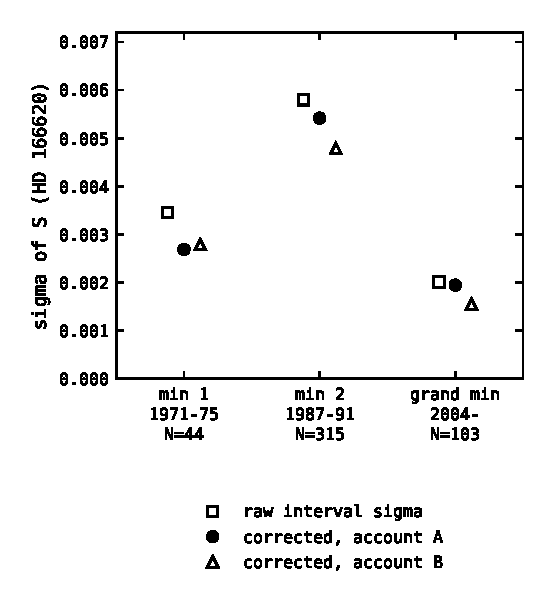
\includegraphics[width=0.6\textwidth]{figures/figure1}
\caption{Variability $\sigma$ of the S index of HD~166620 in three states (data of Luhn et al.). $N$ is the number of observations in the interval. Squares: standard deviation of the whole interval (raw). Circles (method A): interval standard deviation with the instrumental noise variance removed in quadrature. Triangles (method B): mean over seasons of the same corrected value. No uncertainties are shown; the corresponding $F$ tests are in the text.}
\label{fig:h1}
\end{figure}
\begin{figure}[h]
\centering
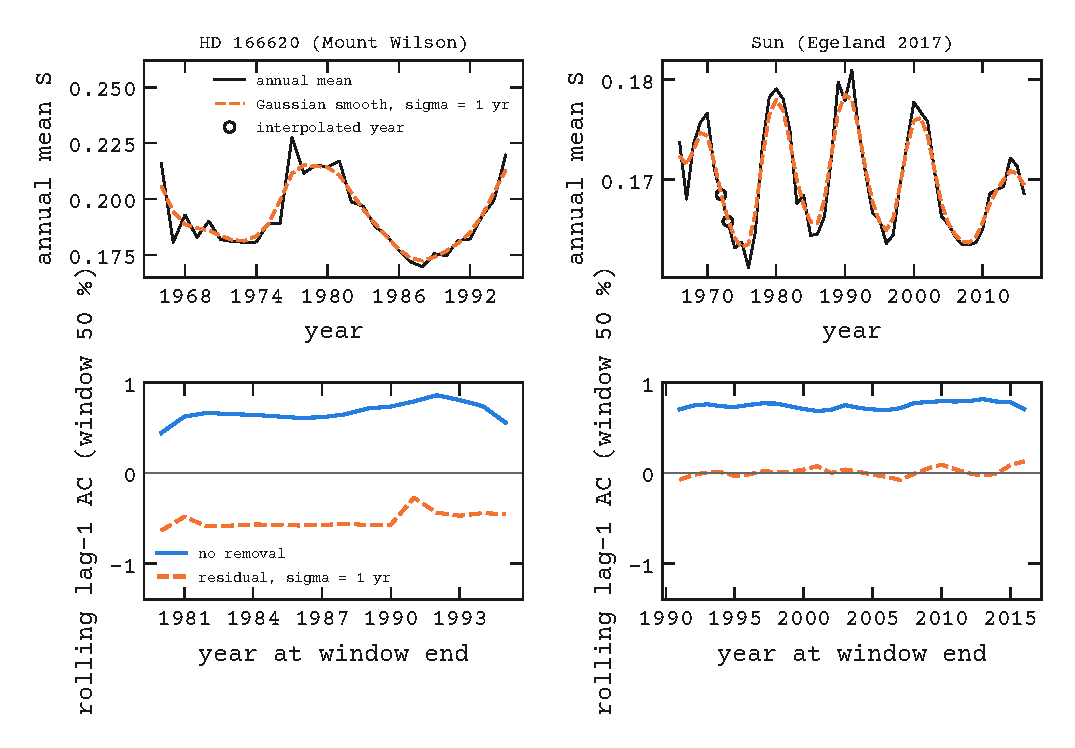
\includegraphics[width=\textwidth]{figures/figure2}
\caption{Top: annual mean S (solid) and its Gaussian smooth with $\sigma = 1$ year (dashed) for HD~166620 (Mount Wilson era) and the Sun (composite series of Egeland et al.; exploratory). Open circles mark interpolated years: none for HD~166620, two for the Sun. The two panels have different vertical ranges. Bottom: rolling lag-1 autocorrelation in a window of 50\,\% of the segment (\WinHD{} years for HD~166620, \WinSun{} for the Sun), plotted at the end year of each window, for the original series (solid) and for the residual, that is, the series minus its smooth (dashed). The horizontal axes share one scale in years.}
\label{fig:roll}
\end{figure}
\begin{figure}[h]
\centering
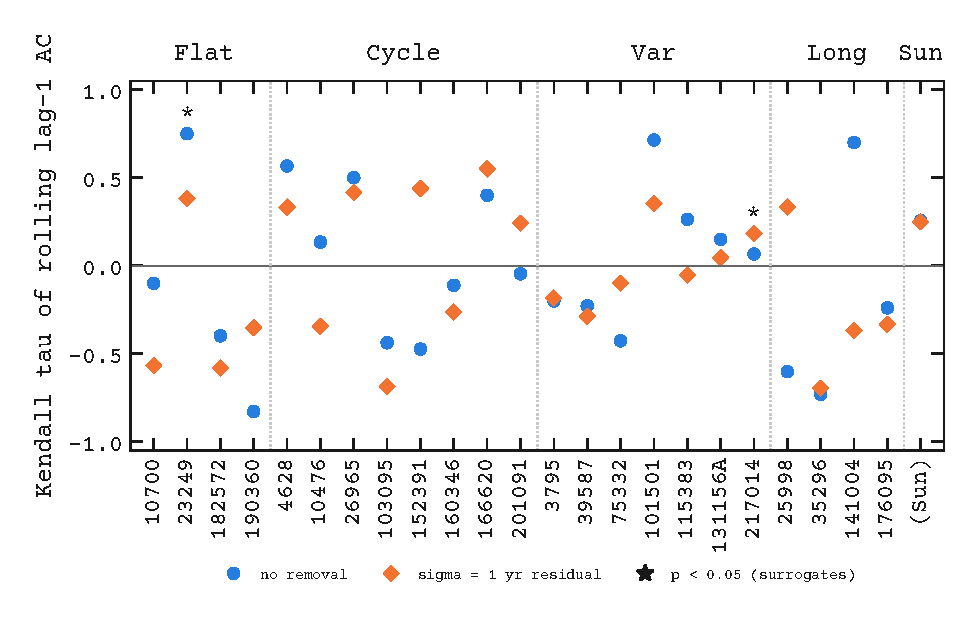
\includegraphics[width=\textwidth]{figures/figure3}
\caption{Kendall $\tau$ of the rolling lag-1 autocorrelation (window of 50\,\% of the longest Mount Wilson segment of each star, annual mean S) for the original series (circles) and the $\sigma = 1$ year residual (diamonds). Stars are grouped as Flat, Cycle, Var and Long and sorted by HD number within a group, which carries no meaning; the Sun (composite series, exploratory) is shown last. An asterisk above a marker means $p < 0.05$ for that configuration, with $p = P(\tau^{*} \ge \tau)$ against the ARMA surrogates (one-sided, upper tail, not corrected for the \NFigTests{} tests shown). The Sun's two markers nearly coincide.}
\label{fig:tau}
\end{figure}
